\documentclass[twoside, a4paper, 12pt, openright, fullpage]{book}
\pagestyle{headings}

\usepackage{import}
\usepackage{mayencourt}
\usepackage[Sonny]{fncychap}

\usepackage[inner=4cm,outer=2cm, top=2cm, bottom=2cm,includeheadfoot]{geometry} 
 
\setlength{\parindent}{0cm}

\title{Cahier 1er année}
\author{Mayencourt Florent}
\date{August 2018}

%%%%%%%%%%%%%%%%%%%%%%%%%%%%%%%%%%%%%%%%%%%%%%%%%
\usepackage{hyperref}

\hypersetup{
backref=true, %permet d'ajouter des liens dans...
 pagebackref=true,%...les bibliographies
hyperindex=true, %ajoute des liens dans les index.
colorlinks=true, %colorise les liens
breaklinks=true, %permet le retour  la ligne dans les liens trop longs
urlcolor= blue, %couleur des hyperliens
linkcolor= blue, %couleur des liens internes
bookmarks=true, %cr des signets pour Acrobat
bookmarksopen=true, %si les signets Acrobat sont crs, les afficher compltement.
pdftitle={Polycopié Math}, %informations apparaissant dans
pdfauthor={Florent MAYENCOURT et Thomas FOURNIER}, %dans les informations du document
pdfsubject={Le cours de mathématiques EC Valais} %sous Acrobat.
}
%%%%%%%%%%%%%%%%%%%%%%%%%%%%%%%%%%%%%%%%%%%%%%%%%%%%

\begin{document}


\begin{titlepage}
\addtolength{\hoffset}{-1cm}
	\centering
	\includegraphics[width=0.50\textwidth]{logo.png}\par\vspace{1cm}
	{\scshape\LARGE Maturité commerciale \par}
	\vspace{1cm}
	{\scshape\Large Recueil d'exercices de révision \par}
	\vspace{1.5cm}
	{\huge\bfseries Mathématiques \par}
	\vspace{2cm}
	{\Large\itshape Sandra \textsc{Roth} et Florent \textsc{Mayencourt} \par}
	\vfill
	supervisé par \par
	professeurs EC \textsc{Martigny}

	\vfill

% Bottom of the page
	{\large \today\par}
\end{titlepage}

\newpage

\tableofcontents

\chapter{Exercices}

\section{Opérations sur les fractions}

\begin{exercice}\label{fraction1}
Effectuer et simplifier si possible :
\begin{multicols}{2}
\begin{enumerate}[a)]
    \item $\displaystyle \frac{2}{7} \cdot \frac{7}{4} = $
    \item $\displaystyle \frac{3}{5} \cdot \frac{15}{9} = $
    \item $\displaystyle 4\cdot  \frac{2}{3} \cdot \frac{5}{2} = $    
    \item $\displaystyle \frac{23}{25} \cdot \frac{125}{69}\cdot 12 = $
    \item $\displaystyle 0.75 \cdot \frac{4}{5} \cdot \frac{12}{7} = $
    \item $\displaystyle \frac{1}{0.75} \cdot0.52 \cdot \frac{12}{5} = $
\end{enumerate}
\end{multicols}
\end{exercice}

\begin{exercice}\label{fraction2}
Effectuer et simplifier si possible :
\begin{multicols}{2}
\begin{enumerate}[a)]
    \item $\displaystyle \frac{3}{4} \div \frac{5}{7} = $
    \item $\displaystyle \frac{-3}{13} \div \frac{5}{26} = $
    \item $\displaystyle \frac{1}{4}\div \left( \frac{6}{7} \div \frac{3}{8}\right) = $
    \item $\displaystyle \frac{20}{3} \div \left(\frac{7}{4}\div \frac{14}{3}\right) = $
    \item $\displaystyle \frac{2}{3} \div \left( \frac{4}{7} \div \frac{16}{3}\right) = $
    \item $\displaystyle \frac{4}{3}\cdot \frac{5}{9} \div \left(\frac{2}{13} \cdot \frac{39}{6}\right) = $
\end{enumerate}
\end{multicols}
\end{exercice}

\begin{exercice}\label{fraction3}
Effectuer et simplifier si possible :
\begin{multicols}{2}
\begin{enumerate}[a)]
    \item $\displaystyle \frac{2}{3}+\frac{4}{3}=$
    \item $\displaystyle \frac{8}{5}-\frac{3}{5}$
    \item $\displaystyle\frac{1}{2}-\frac{1}{3}+\frac{1}{4}=$
    \item $\displaystyle\frac{2}{5}+\frac{1}{16}+\frac{1}{20}=$
    \item $\displaystyle \frac{2}{5}+\frac{1}{2}-\frac{4}{3}=$
    \item $\displaystyle \frac{5}{14}-\frac{2}{35}+\frac{3}{70}-\frac{2}{7}=$
    \item $\displaystyle\frac{5}{6}+\left(-\frac{4}{5}\right) - \left(-\frac{2}{15}\right)=$
    \item $\displaystyle\frac{1}{6}-\frac{2}{-7}+\frac{-3}{8}=$
    \item $\displaystyle \frac{5}{18}-\frac{7}{6}+\frac{3}{9}-2=$
    \item $\displaystyle 2-\frac{13}{7}+\left(1+\frac{5}{2}\right)=$
    \end{enumerate}
\end{multicols}
\end{exercice}

\subsection{Exercices supplémentaires}

\begin{exercice}\label{fraction4}
Effectuer et simplifier si possible :
\begin{multicols}{2}
\begin{enumerate}[a)]
    \item $\displaystyle \left(\frac{2}{3} -\frac{3}{4}\right) \div \frac{5}{6}$
    \item $\displaystyle 12-2\cdot \left( -\frac{3}{8}+\frac{4}{5}\right) \cdot 4$
    \item $\displaystyle \frac{5}{4}+\frac{1}{3}\div \frac{3}{5}-\frac{11}{12}\cdot \frac{2}{3}$
    \item $\displaystyle 5\cdot \frac{2}{5}\cdot \frac{1}{6}+\frac{3}{2}\div \frac{2}{7}$
    \item $\displaystyle  \left( \frac{4}{7}-\frac{3}{5}+\frac{5}{6}\right) \cdot \frac{15}{26}-\frac{3}{7}$
    \item $\displaystyle \frac{22}{9}-\frac{1}{3}\cdot \frac{4}{3}\div \frac{5}{6}-\frac{2}{5}$
    \item $\displaystyle \left(\frac{2}{3}-\frac{3}{4}\right) + 3\cdot \left( \frac{4}{5}-\frac{5}{6}\right)$
    \item $\displaystyle \left( \frac{1}{2}+\frac{5}{3}\right) \cdot \left( 3+\frac{7}{4}\right) \div \left( \frac{1}{2}-\frac{5}{6}\right)$
    \end{enumerate}
\end{multicols}
\end{exercice}

\begin{exercice}\label{fraction5}
Effectuer et simplifier si possible :
\begin{multicols}{2}
\begin{enumerate}[a)]
    \item $\displaystyle \frac{\frac{1}{3}+\frac{1}{2}-\frac{3}{7}}{\frac{2}{3}-\frac{4}{7}+\frac{1}{6}}$
    \item $\displaystyle \frac{\frac{1}{5}-\frac{1}{15}+\frac{5}{25}}{\frac{26}{36}+\frac{1}{6}-\frac{2}{9}}$
    \item $\displaystyle \frac{3\div\frac{3}{4}}{\frac{5}{7}\div 7}$
    \item $\displaystyle \frac{\frac{1}{4}\div\left(\frac{6}{7}\div\frac{3}{8}\right)}{\left(\frac{3}{4}\div\frac{4}{5}\right) \cdot \frac{8}{5}}$
    \item $\displaystyle \frac{\left(\frac{11}{3}\div \frac{9}{22}\right) \cdot \frac{6}{121}}{\left(\frac{1}{3}-\frac{5}{23}\right)\cdot \left(\frac{4}{3}-\frac{3}{8}\right)}$
    \item $\displaystyle \frac{2\cdot \left(\frac{3}{2}+\frac{1}{2}\cdot \frac{15}{4}\right)}{3\cdot \left(\frac{54}{12}\cdot \frac{21}{5}\cdot \frac{10}{6}\right)}$
    \end{enumerate}
\end{multicols}
\end{exercice}

\section{Calculs de puissances}

\begin{exercice}\label{puissances1}
Réduire les expressions suivantes :
\begin{multicols}{2}
\begin{enumerate}[a)]
    \item $4^2 \cdot 4^2$
    \item $10^3\cdot 10^4$
    \item $10^5 \cdot 10^{-3}$
    \item $5^4\cdot 5^{-4}$
    \item $5^4\div 5^1$
    \item $3^4\div 3^2$
    \item $4^4\div 4^{-2}$
    \item $10^2\div 10^{-4}$
    \item $\left(4^5\right)^2$
    \item $\left(3^2\right)^2$
    \item $\left(10^2\right)^{-1}$
    \item $\left(5^{-4}\right)^{-3}$
    \end{enumerate}
\end{multicols}
\end{exercice}

\begin{exercice}\label{puissances2}
Réduire les expressions suivantes :
\begin{multicols}{2}
\begin{enumerate}[a)]
    \item $\left(10^{-2}\cdot 10^4\right)^5$
    \item $\left(5^{-4}\cdot 5^5\right)^5$
    \item $\left(3^3\right)^3 \cdot 3^2$
    \item $\left(4^1\right)^2 \cdot 4^3$
    \item $\left(4^2\cdot 4^3\right) \div 4^{-1}$
    \item $\left(2^1\cdot 2^1\right) \div 2^{-4}$
    \item $10^3 \div \left(10^3 \cdot 10^3 \right)$
    \item $3^5 \div \left(3^3 \cdot 3^4\right)$
    \end{enumerate}
\end{multicols}
\end{exercice}

\begin{exercice}\label{puissances3}
Réduire les expressions suivantes :
\begin{multicols}{2}
\begin{enumerate}[a)]
    \item $\left(3^2 \cdot 3^{-4}\right) \div \left(3^2\cdot 3^2\right)$
    \item $\left(10^3 \cdot 10^3 \right) \div \left(10^{-3}\cdot 10^2\right)$
    \item $\left(5^5 \cdot 5^5 \cdot 5^3\right) \div \left(5^3\cdot 5^1\right)$
    \item $\left(2^1 \cdot 2^3 \cdot 2^3\right) \div \left( 2^2 \cdot 2^4 \right)$
    \item $\left(3^2 \cdot \left(3^3\right)^2\right) \div \left(3^2\right)^2$
    \item $\left(4^3\left(4^2\right)^3\right) \div \left(4^1\right)^4$
    \item $2^3 \div \left(\left(2^{-3}\right)^1 \cdot 2^1\right)$
    \item $10^{-3} \div \left(\left(10^{-3}\right)^4 \cdot 10^1\right)$
    \end{enumerate}
\end{multicols}
\end{exercice}

\section{Calculs de racines}

\begin{exercice}\label{racines1}
Effectuer les opérations suivantes :
\begin{multicols}{2}
\begin{enumerate}[a)]
    \item $\sqrt{36 \cdot 25}$
    \item $\sqrt{9\cdot 25 \cdot 7}$
    \item $\sqrt{2^4 \cdot 3^6}$
    \item $\sqrt{2^3 \cdot 3^4 \cdot 5^6}$
    \item $\sqrt{5}\cdot \sqrt{15}$
    \item $\sqrt{6}\cdot \sqrt{24}$
    \item $\sqrt{32}\cdot \sqrt{2}$
    \item $\sqrt{8}\cdot \sqrt{18}$
    \item $\sqrt{0.04} \cdot \sqrt{24}$
    \item $\sqrt{7.5}\cdot \sqrt{30} \cdot \sqrt{0.09}$
    \item $\sqrt[3]{5\cdot 3^3}$
    \item $\sqrt[5]{2^5 \cdot 3^5}$
    \item $\sqrt[3]{4} \cdot \sqrt[3]{18}$
    \item $\sqrt[3]{9}\cdot \sqrt[3]{3}$
    \end{enumerate}
\end{multicols}
\end{exercice}

\begin{exercice}\label{racines2}
Effectuer les opérations suivantes :
\begin{multicols}{4}
\begin{enumerate}[a)]
    \item $\sqrt{\frac{9}{16}}$
    \item $\sqrt{\frac{4}{81}}$
    \item $\sqrt{\frac{32}{9}}$
    \item $\sqrt{\frac{48}{169}}$
    \item $\frac{\sqrt{2}}{\sqrt{8}}$
    \item $\frac{\sqrt{6}}{\sqrt{75}}$
    \item $\frac{\sqrt{50}}{\sqrt{18}}$
    \item $\frac{\sqrt{14}}{\sqrt{63}}$
    \end{enumerate}
\end{multicols}
\end{exercice}

\begin{exercice}\label{racines3}
Effectuer les opérations suivantes :
\begin{multicols}{2}
\begin{enumerate}[a)]
    \item $\left( \sqrt{5} \cdot \sqrt{3}\right)^2$
    \item $\left(  \sqrt{2} \cdot \sqrt{3}\right)^4$
    \item $\sqrt{\sqrt{162}}$
    \item $\sqrt{\sqrt[3]{64}}$
    \item $\sqrt{\sqrt{5}}\cdot \sqrt{5\cdot \sqrt{5}}$
    \item $\sqrt{6\cdot \sqrt{2}}\cdot \sqrt{3\cdot \sqrt{2}}$
    \end{enumerate}
\end{multicols}
\end{exercice}

\section{Calcul littéral}

\begin{exercice}\label{littéral1}
Simplifier les expressions suivantes :
\begin{multicols}{2}
\begin{enumerate}[a)]
    \item $-2\cdot \left( x^2\right) ^2$
    \item $-7\cdot \left(-x^3\right)^2$
    \item $-5\cdot \left( x^2y \right)^4$
    \item $6\cdot \left(-2xy^3\right)^4$
    \item $\left(-2x^3\right)^2 \cdot 3x^4$
    \item $\left(-6x^2\right) \cdot 2x^3 \cdot \left(-x\right)^5$
    \item $-\left(3x^3y\right)^2 \cdot 2\left(xy^2\right)^3$
    \item $\left(0.1 x^2y\right)^3 \cdot \left(10x^3y^2\right)2$
    \item $\left(-5y^4\right)\cdot \left(2xy^2\right) \cdot\left(-6x^{-2}y\right)$
    \item $\left(x^2yz^3\right) \cdot \left(-2xz^2\right)\cdot \left(6x^3y^{-2}\right)$
    \item $\left(\frac{2}{3}x^2y^{-3}\right) \cdot \left(-\frac{3}{5}xy^2\right) \cdot \left(25x^{-1}y^2\right)$
    \item $\left(\frac{1}{2}x^2y^{-5} \right) \cdot \left(6x^{-3}y\right) \cdot \left(\frac{1}{3}x^{-1}y^3\right)$
    \end{enumerate}
\end{multicols}
\end{exercice}

\begin{exercice}\label{littéral2}
Effectuer, réduire et ordonner :
\begin{multicols}{2}
\begin{enumerate}[a)]
    \item $20x-\left(16x-\left(2x+y\right)\right)$
    \item $15x-\left(5x-\left(2x-y\right)\right)$
    \item $(x-1)\cdot \left(2x-x^2+4\right)$
    \item $\left(1-3x^2+5x^3\right) \cdot (x-1)$
    \item $\left(3y-1\right)\cdot \left(4y^2-5y+6\right)$
    \item $\left(6z^2-3z-4\right) \cdot \left(5z-3\right)$
    \item $\left(x-2\right) \cdot \left(x+3\right) \cdot \left(x+5\right)$
    \item $\left(2x+1\right) \cdot \left(3x-1\right) \cdot \left(5x+2\right)$
    \item $\left( 2x-5\right) \cdot \left(3y-7\right)$
    \item $\left(-3x-2y\right)\cdot \left(-x-y\right)$
    \item $\left(3z-5\right)\cdot \left(2y+7\right)$
    \item $\left(9z-2\right) \cdot \left(3-4y\right)$
    \item $\left(-2-y\right) \cdot \left(z+2 \right) \cdot 4x$
    \item $-2y\cdot \left( 3-2x\right) \cdot \left( 2x-y\right)$
    \end{enumerate}
\end{multicols}
\end{exercice}

\section{Fractions et équations rationnelles}

\begin{exercice}\label{fraction6}
Effectuer les opérations suivantes :
\begin{multicols}{2}
\begin{enumerate}[a)]
    \item $\displaystyle \frac{1}{x}+\frac{1}{3x}$
    \item $\displaystyle \frac{1}{x-1}-\frac{1}{2x-2}$
    \item $\displaystyle \frac{3}{x-3}-\frac{2}{x-2}$
    \item $\displaystyle \frac{2}{x-6}+\frac{1}{2x+3}$
    \item $\displaystyle \frac{1}{x-2}-\frac{4}{x^2-4}$
    \item $\displaystyle \frac{2x^2+4x-2}{x^2+2x-3}-\frac{2x-1}{x-1}$
    \item $\displaystyle \frac{x+3}{2x+12}\cdot \frac{x^2-36}{x^2+6x+9}$
    \item $\displaystyle \frac{9x^2-9-54}{x^2+2x-3}\cdot \frac{x^2-1}{3x-9}$
    \item $\displaystyle \frac{7x+2}{4x^3}\div \frac{49x^2-4}{8x}$
    \item $\displaystyle \frac{-3x}{x-2}\div \frac{12}{10-5x}$
    \end{enumerate}
\end{multicols}
\end{exercice}

\begin{exercice}\label{fraction7}
Effectuer les opérations suivantes :
\begin{multicols}{2}
\begin{enumerate}[a)]
    \item $\displaystyle \frac{x+1}{x-4}=0$
    \item $\displaystyle \frac{3-2x}{4-3x}=0$
    \item $\displaystyle \frac{x+1}{x-2}=\frac{x-3}{x+4}$
    \item $\displaystyle \frac{5+2x}{1-4x}= \frac{x+3}{5-2x}$
    \item $\displaystyle \frac{x-3}{x+3}-\frac{x+3}{x-3}= \frac{3}{x^2-9}$
    \item $\displaystyle \frac{3x+1}{x+1}-\frac{2x}{x+2}= -\frac{4}{x^2+3x+2}$
    \item $\displaystyle \frac{x-1}{x-2}=\frac{x-3}{x-4}$
    \item $\displaystyle \frac{x}{x+1}-\frac{2}{x}= \frac{x^2}{x^2 + x}$
    \item $\displaystyle \frac{3x+1}{3\cdot (x-3)}+ \frac{2x+1}{2\cdot (x+3)} = 2$
    \item $\displaystyle \frac{5}{x-3}-\frac{2}{x-4}= \frac{3}{x-5}$
    \end{enumerate}
\end{multicols}
\end{exercice}

\section{Systèmes $2\times 2$}

\begin{exercice}\label{systeme}
\begin{multicols}{2}
\begin{enumerate}[a)] Résoudre les systèmes suivants :
    \item $$
            \left\{
            \begin{array}{ll}
               \displaystyle x+\frac{3y}{7}  &=17  \\
               \\
                \displaystyle y-\frac{5x}{8} &=16 
            \end{array}
            \right.
            $$
    \item $$
    \left\{
            \begin{array}{ll}
              \displaystyle  \frac{x}{3}+\frac{y}{4}  &=9  \\
            \\
            \displaystyle \frac{x}{4}+\frac{y}{5} &=7 
            \end{array}
            \right.
            $$
    \item $$
    \left\{
            \begin{array}{ll}
             \displaystyle   \frac{4x-5}{2y-3}  &=3  \\
             \\
             \displaystyle    \frac{3x+5}{y+1} &=4 
            \end{array}
            \right.
            $$
    \item $$
            \left\{
            \begin{array}{ll}
             \displaystyle   \frac{x-1}{8}+\frac{y-2}{5}  &=2  \\
             \\
             \displaystyle    2x+\frac{2y-5}{3} &=21 
            \end{array}
            \right.
            $$
    \item $$
            \left\{
            \begin{array}{ll}
             \displaystyle   \frac{x-4}{3} -\frac{3y+4}{10} &=x-y  \\
             \\
             \displaystyle    \frac{2x-5}{5}-\frac{2y-4}{4} &=x-12 
            \end{array}
            \right.
            $$
    \item $$
            \left\{
            \begin{array}{ll}
              \displaystyle  \frac{4x+15}{3}-\frac{3y-5}{5}  &=x  \\
              \\
              \displaystyle   \frac{2y+3x}{4}+\frac{y+15}{5} &=y 
            \end{array}
            \right.
            $$
    \item $$
            \left\{
            \begin{array}{ll}
             \displaystyle   \frac{x-y}{3}-\frac{1}{4}\left(x-\frac{10-2y}{3}\right)  &=3  \\
             \\
             \displaystyle    \frac{x-5y}{5}+\frac{x+2}{2}&=x-4 
            \end{array}
            \right.
            $$
    \item $$
            \left\{
            \begin{array}{ll}
             \displaystyle   \frac{3x}{5}+\frac{4y}{10}  &=\frac{x-y}{5}  \\
             \\
              \displaystyle   \frac{10(2x+3)}{11}-2\left(y-\frac{3x-5}{8}\right) &=60 
            \end{array}
            \right.
            $$
    \item $$
            \left\{
            \begin{array}{ll}
              \displaystyle  \frac{13}{3+x+2y}+\frac{3}{6+4x-5y}  &=0  \\
              \\
              \displaystyle   \frac{6x-5y+4}{3} &=\frac{3x+2y+1}{19} 
            \end{array}
            \right.
            $$
    \item $$
            \left\{
            \begin{array}{ll}
              \displaystyle  \frac{x+5}{x+1}  &=\frac{y-9}{y+7}+\frac{112}{(x+1)(y+7)}  \\
              \\
              \displaystyle   2x+10 &=3y+1 
            \end{array}
            \right.
            $$
    \end{enumerate}
\end{multicols}
\end{exercice}

\section{Inéquations}

\begin{exercice}\label{inequations}
\begin{multicols}{2}
\begin{enumerate}[a)]
\item $7x-6>5+6x$
\item $12-5x>x-60$
\item $ \frac{x}{3}+\frac{x}{2}>\frac{4}{x}+\frac{1}{2}$
\item $ \frac{x}{2}+4 >\frac{2x}{3}-\frac{x}{8}$
\item $4(5+x) >5(x+3)$
\item $3-4(5-x) \leq 2x+5$
\item $\frac{3x-1}{5}-\frac{13}{2} \geq \frac{7x}{3}-\frac{11(x+3)}{6}$
\item $4(x^2+1)+8(3x-4)>4x^2$
\item $\frac{x-5}{3}-\frac{x-8}{4}\leq 0$
\item $\frac{5x}{3}+1-\frac{8x+1}{4}>0$
\item $\frac{3x}{2}-\frac{2x}{3}\geq 5\left(\frac{x}{6}+1\right) -5$
\item $\frac{3x}{2}-\frac{2x}{3}> 5\left(\frac{x}{6}+1\right) -5$
\item $(3x+45)(3x+3)<(3x+6)(3x+18)$
\item $\frac{6x-1}{12}-\frac{3}{4}\geq 4x-\frac{5(1-4x)}{2}$
\item $2x-\frac{6x+1}{2}-\frac{8x-1}{3}+\frac{11x}{3}<0$
\item $\frac{(3x-7)(3x+7)}{6}<\frac{(x-2)^2}{2}+\frac{(2x+1)^2}{4}$
\item $2x-\frac{2x}{9}\leq \frac{1}{9}\left(16x-\frac{3}{2}\right)$
\item $\frac{-x+1}{3}-\frac{-x-1}{4}\geq \frac{x}{2}+\frac{2+x}{24}$
\item $\frac{(x+1)^2}{16}-\frac{1+x}{2}<\frac{(x-1)^2}{16}-\frac{2+x}{4}$
\end{enumerate}
\end{multicols}
\end{exercice}

\section{Mensualités}

\begin{exercice}\label{mensualite1}
Quelle somme aurez-vous sur votre compte privé si vous versez CHF 550.- chaque fin du mois au taux de $1.3\%$, capitalisation mensuelle, pendant $13$ ans ?
\end{exercice}

\begin{exercice}\label{mensualite2}
Vous désirez disposer de CHF 17'000.- sur votre compte en banque dans 7 ans. Si le taux est à $1.4\%$, combien devez-vous déposer en banque à chaque fin de mois ? chaque fin de trimestre ?
\end{exercice}

\begin{exercice}\label{mensualite3}
Chaque fin de mois, on dépose CHF 500.- sur un compte où le taux d'intérêt est de $0.75\%$, capitalisation mensuelle. Combien de mensualité doit-on verser pour obtenir au moins CHF 25'000.- ?
\end{exercice}

\begin{exercice}\label{mensualite4} %partie a) pas dans le PEC
Un dette de CHF 150'000.- contractée pendant 10 ans à capitalisation trimestrielle a coûté, capital et intérêt compris, CHF 223'329.56 :
\begin{enumerate}[a)]
    \item A quel taux annuel cette dette avait-elle été contractée ? (réponse en $\%$, arrondir si nécessaire)
\end{enumerate}
Si le taux de cet emprunt de CHF 150'000.- avait été de $3.8\%$, capitalisation trimestrielle :
\begin{enumerate}[a)]
\setcounter{enumi}{1}
    \item Quelles annuités trimestrielles aurait-il fallu verser à  la banque pour amortir totalement cette dette en 8 ans ?
\end{enumerate}
\end{exercice}

\begin{exercice}\label{mensualite5}
Au lieu de payer un loyer, une famille décide d'acheter un appartement. Cette famille peut verser trimestriellement CHF 3'750.- comme annuité. Si le taux hypothécaire à ce jour est de $3.75\%$, capitalisation trimestrielle, et que cette famille veut totalement amortir sa dette en $25$ans : Quel montant maximal pourra-t-elle emprunter aujourd'hui ? (arrondir le montant au franc)
\end{exercice}

\section{Calculs divers}

\begin{exercice}\label{exercice1}
Résoudre pour $x$ en donnant le domaine de définition de l'équation
\begin{multicols}{2}
\begin{enumerate}[a)]
\item
$$
2\cdot 3^{2x-1}  =  5 \cdot 2^{3+x}
$$
\item
$$
\sqrt[x-3]{7^x}  =  23
$$
\item
$$
\log(2x+1) - 2\log(x-4) = 1
$$
\item
$$
\log(x+1)+\log(x-3) = 2 + 2\log(x-1)
$$
\item
$$
\frac{x-2}{x+3} - \frac{2}{x-3} = \frac{2x^2}{x^2-9}
$$
\item
$$
\frac{1}{x-2} - \frac{1}{x+2} = \frac{1}{35}
$$
\item
$$
x-7 = 6-(x-7)^2
$$
\item 
$$
(x+3)^2 - (x-4)^2 = 721
$$
\item 
$$
3(5x-8) = 4(5x+7)-1
$$
\item 
$$
\frac{2x+3}{4} - \frac{1}{5} = \frac{3-x}{6}
$$ 
\end{enumerate}
\end{multicols}
\end{exercice}

\section{Programmation linéaire}

\begin{exercice}\label{exercice2}
Pour décorer l'école, vous avez besoin d'au moins $1200$ lampions, $3000$ étoiles et $2400$ sapins en carton.

Dans un premier magasin, vous trouvez l'offre suivante pour 15 frs :
\begin{itemize}
\item 3 lampions
\item 5 étoiles
\item 3 sapins en carton
\end{itemize}
Tandis que dans un second magasin, vous trouvez l'offre suivante pour 14 frs : 
\begin{itemize}
\item 2 lampions
\item 6 étoiles
\item 8 sapins en carton
\end{itemize}


\begin{enumerate}[(a)]
\item Déterminez la manière d'acheter les décorations pour minimiser les coûts.\label{item1}
\item Pouvez-vous respecter le budget de 8000 frs qui vous a été confié ? Si oui, combien vous reste-t-il ?
\item Une fois les offres achetées selon la réponse (\ref{item1}), quel est votre stock de lampions, étoiles et sapins en carton ?
\item Au moment de vous rendre dans le premier magasin, vous remarquer qu'il fait un rabais de 10 frs sur les décorations (qui sont donc vendues à 5 frs). Que faites-vous ?
\end{enumerate}
\end{exercice}

% CB a rajouté un exemple
\begin{exercice}\label{exercice2}
Un atelier de confection fabrique deux modèles de robes. L’un exige 3m de tissu et 30h de travail, il procure un bénéfice de Fr. 50.— par robe. L’autre exige 3,5m de tissu et 15h de travail, il procure un bénéfice de Fr. 35.— par robe.

\begin{enumerate}[(a)]
\item Sachant que l’atelier dispose de 200m de tissu et de 1200h de travail par jour, quelle quantité de chaque modèle faut-il fabriquer pour que le bénéfice quotidien soit maximum ?
\item Quel est ce bénéfice ?
\end{enumerate}
\end{exercice}

\section{Statistiques}
\begin{exercice}
On a relevé le nombre de pièces dans les logements d’une ville de la région et obtenu les valeurs suivantes :
\begin{center}
\begin{tabular}{|l|l|l|l|l|l|l|l|l|l|l|l|}
\hline
2&3&5&3&4&4&3&4&1&2&6&2 \\ \hline
2&2&1&1&5&2&2&6&3&1&2&2     \\ \hline
4&1&2&6&4&5&2&1&2&3&2&3    \\ \hline
\end{tabular}
\end{center}

\begin{enumerate}[(a)]
\item Établir un tableau statistique comprenant le temps d'attente, le centre de classe, l’effectif, la fréquence, la fréquence cumulée, la fréquence cumulée inverse, la fréquence pondérée et la fréquence pondérée au carrée.
Précision des calculs : 2 chiffres après la virgule.
\item Établir l'histogramme des effectifs et des fréquences cumulées.
\item Indiquer le mode et la médiane de cette distribution statistique.
\item Calculer la moyenne et l'écart type

\end{enumerate}
\end{exercice}


\chapter{Solutions}
\section{Opérations sur les fractions}
\subsection{Exercices supplémentaires}

\section{Calculs de puissances}

\section{Calculs divers}
\begin{solutions}{\ref{exercice1}}
\begin{multicols}{2}
\begin{enumerate}[a)]
\item $\displaystyle x=\frac{\log(60)}{\log(9/2)} \simeq 2.72216 $
\item
$\displaystyle x = \frac{3 \log(23)}{\log(23/7)} \simeq 7.90737$
\item
$\displaystyle S= \{\frac{41-\sqrt{91}}{10};\frac{41+\sqrt{91}}{10}\}$
\item
$S=\emptyset$
\item
$S=\{-7;0\}$
\item
$S=\{-12;12\}$
\item
$S=\{4;9\}$
\item 
$S=\{52\}$
\item 
$S=\{-\frac{51}{5}\}$
\item 
$S=\{-\frac{3}{40}\}$
\end{enumerate}
\end{multicols}
\end{solutions}

\section{Programmation linéaire}

\begin{solutions}{\ref{exercice2}}

\begin{tabular}{|l|l|l|l|}
\hline
 & Premier Magasin & Deuxième magasin & Contraintes \\ \hline
Lampions & 3  & 2    & 1200     \\ \hline
Étoiles& 5  & 6    & 3000     \\ \hline
Sapins  & 3  & 8   & 2400      \\ \hline
Prix de vente   & 15 frs  & 14 frs  & Minimum    \\ \hline
\end{tabular}


Système d’inéquation : $\left\{ \begin{array}{ll}
  & x\ge 0 \\ 
 & y\ge 0 \\ 
 & 3x+2y\geq 1200 \\ 
 & 5x+6y\geq 3000 \\ 
 & 3x+8y\geq 2400 \\ 
\end{array} \right.$

avec $15x+14y=\,\,\text{minimum}$

Étude des droites limites : 

${{d}_{1}}:2x+3y=1200\,\,\,\left| \begin{array}{ll}
  & pente\,\,{{a}_{1}}=-\frac{2}{3} \\ 
 & ord.\,\,or.\,\,:x=0\Rightarrow y=400 \\ 
 & z\acute{e}ro\,\,fct\,\,:y=0\Rightarrow x=600 \\ 
\end{array} \right.$  

${{d}_{2}}:5x+6y=3000\,\,\,\left| \begin{array}{ll}
  & pente\,\,{{a}_{2}}=-\frac{5}{6} \\ 
 & ord.\,\,or.\,\,:x=0\Rightarrow y=500 \\ 
 & z\acute{e}ro\,\,fct\,\,:y=0\Rightarrow x=600 \\ 
\end{array} \right.$

${{d}_{3}}:3x+8y=2400\,\,\,\left| \begin{array}{ll}
  & pente\,\,{{a}_{3}}=-\frac{3}{8} \\ 
 & ord.\,\,or.\,\,:x=0\Rightarrow y=300 \\ 
 & z\acute{e}ro\,\,fct\,\,:y=0\Rightarrow x=800 \\ 
\end{array} \right.$  

${{d}_{M}}:15x+14y=M\,\,:\,\,pente\,\,{{a}_{M}}=-\frac{15}{14}$

Graphique :

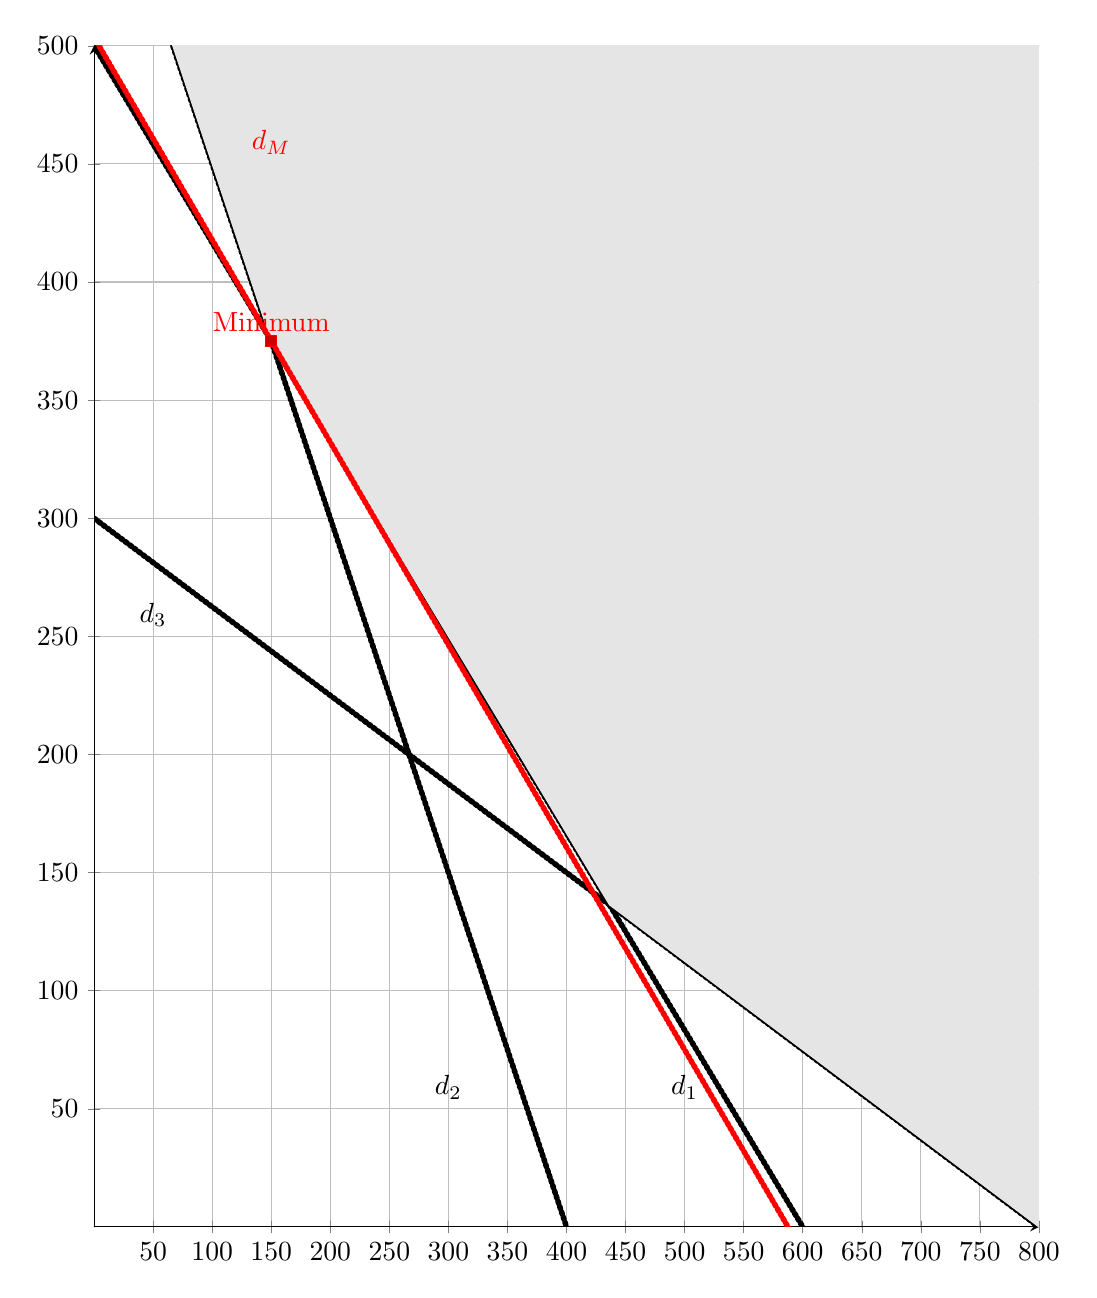
\begin{tikzpicture}[line cap=round,line join=round,x=1cm,y=1cm]
\begin{axis}[
x=0.15mm,y=0.3mm,
axis lines=middle,
ymajorgrids=true,
xmajorgrids=true,
xmin=0,
xmax=800,
ymin=0,
ymax=500,
xtick={0,50,...,800},
ytick={0,50,...,500},
]
\draw [line width=2pt,dash pattern=on 1pt off 1pt,domain=0:800] plot(\x,{(1200-3*\x)/2});
\node[above](d_1) at (500,50) {$d_1$};
\draw [line width=2pt,dash pattern=on 1pt off 1pt,domain=0:800] plot(\x,{(3000-5*\x)/6}) ;
\node[above](d_2) at (300,50) {$d_2$};
\draw [line width=2pt,dash pattern=on 1pt off 1pt,domain=0:800] plot(\x,{(2400-3*\x)/8});
\node[above](d_3) at (50,250){$d_3$};
\addplot[fill, color=gray!20] coordinates {(0,600) (150,375) (4800/11,1500/11) (800,0) (800,600)};
\addplot+[only marks, point meta = explicit symbolic, nodes near coords] coordinates {(150,375)[Minimum]};
\draw [line width=2pt,dash pattern=on 1pt off 1pt,domain=0:800, color=red] plot(\x,{(7050-12*\x)/14});
\node[above, color=red](d_m) at (150,450){$d_M$};
\end{axis}
\end{tikzpicture}

Résolution algébrique : $\left\{ \begin{array}{ll}
  & 5x+6y=3000 \\ 
 &  3x+8y=2400\\ 
\end{array} \right.\Rightarrow \left\{ \begin{array}{ll}
  & x= 150\\ 
 & y= 375\\ 
\end{array} \right.$

Recette maximale : $12 \cdot 150+14 \cdot 375= 7050$
\end{solutions}

\end{document}
